% =========================================================================
%
%
% =========================================================================
% !TeX TXS-program:compile = txs:///pdflatex/[--shell-escape]
\documentclass[aspectratio=1610]{beamer}

% ========================= Theme =========================================
\usetheme{CambridgeUS}
\usecolortheme{default}

% ========================= Packages ======================================
\usepackage{calc}
\usepackage{tikz}
\usetikzlibrary{arrows,
arrows.meta,
calc,
chains,
quotes,
positioning,
shapes,
shapes.geometric}
\usepackage{graphicx}
\usepackage{graphics}
\usepackage{pgfplots}
\pgfplotsset{width=7cm,compat=1.17}

%% ========================== Coding snippets =============================
% Default fixed font does not support bold face
\usepackage{minted}

% ========================= Infor on authors ==============================
\title{Intro to Python --- SMM692}
\subtitle{Getting Started with Python}
\author{Simone Santoni}
\institute{Bayes Business School}
\date{MSc Pre-Course Series}

% ============================ Colors =====================================
\definecolor{base_c}{rgb}{0.6,0,0}
\definecolor{comp_c}{rgb}{0.09803921568627451, 0.6901960784313725, 0.7529411764705882}
\definecolor{tri_1}{rgb}{0.09803921568627451, 0.7686274509803922, 0.19215686274509805}
\definecolor{tri_2}{rgb}{0.19215686274509805, 0.09803921568627451, 0.7686274509803922}

% ========================= TOC  ==========================================
\AtBeginSubsection[]
{
    \begin{frame}
        \frametitle{Outline}
        \tableofcontents[currentsection,currentsubsection]
    \end{frame}
}

% ========================= Document  ====================================
\begin{document}

\begin{frame}
	\titlepage
\end{frame}

\begin{frame}{Outline}
	\tableofcontents
\end{frame}

% ------------------------- Background -----------------------------------

\section{Installing Python}

\subsection{Options}

\begin{frame}[c]{Option 1: Official Installer}
	\begin{figure}
		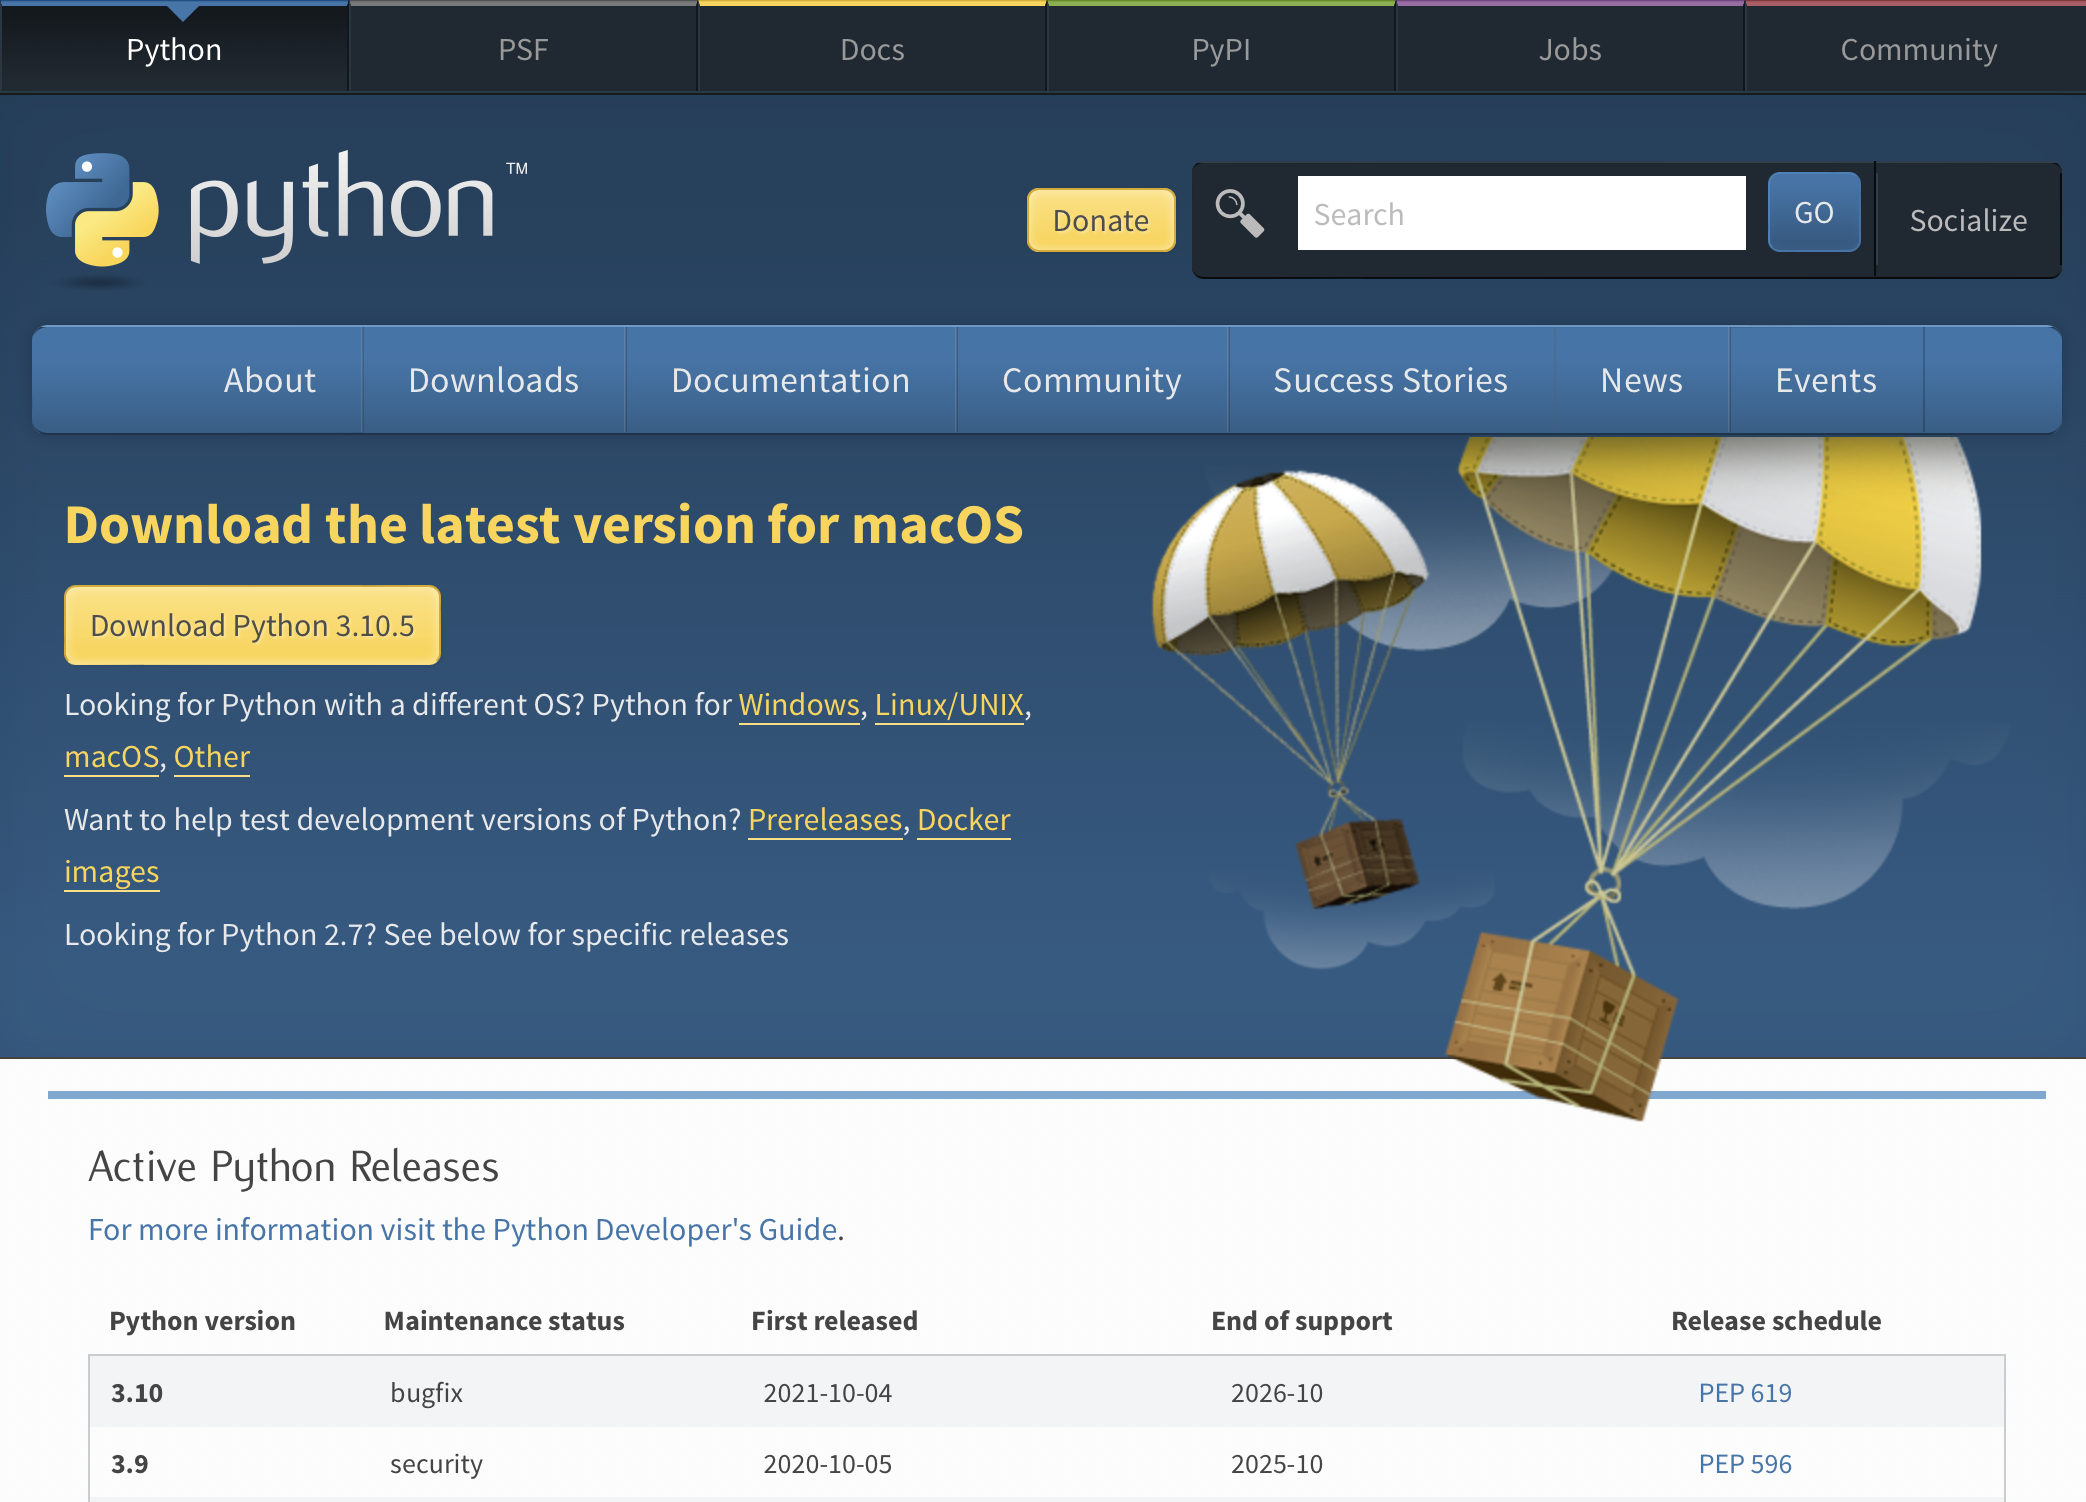
\includegraphics[width=0.75\textwidth]{images/official_installer.png}
	\end{figure}
\end{frame}

\begin{frame}[c]{Option 2: Anaconda Distro (Preffered Way)}
	\begin{figure}
		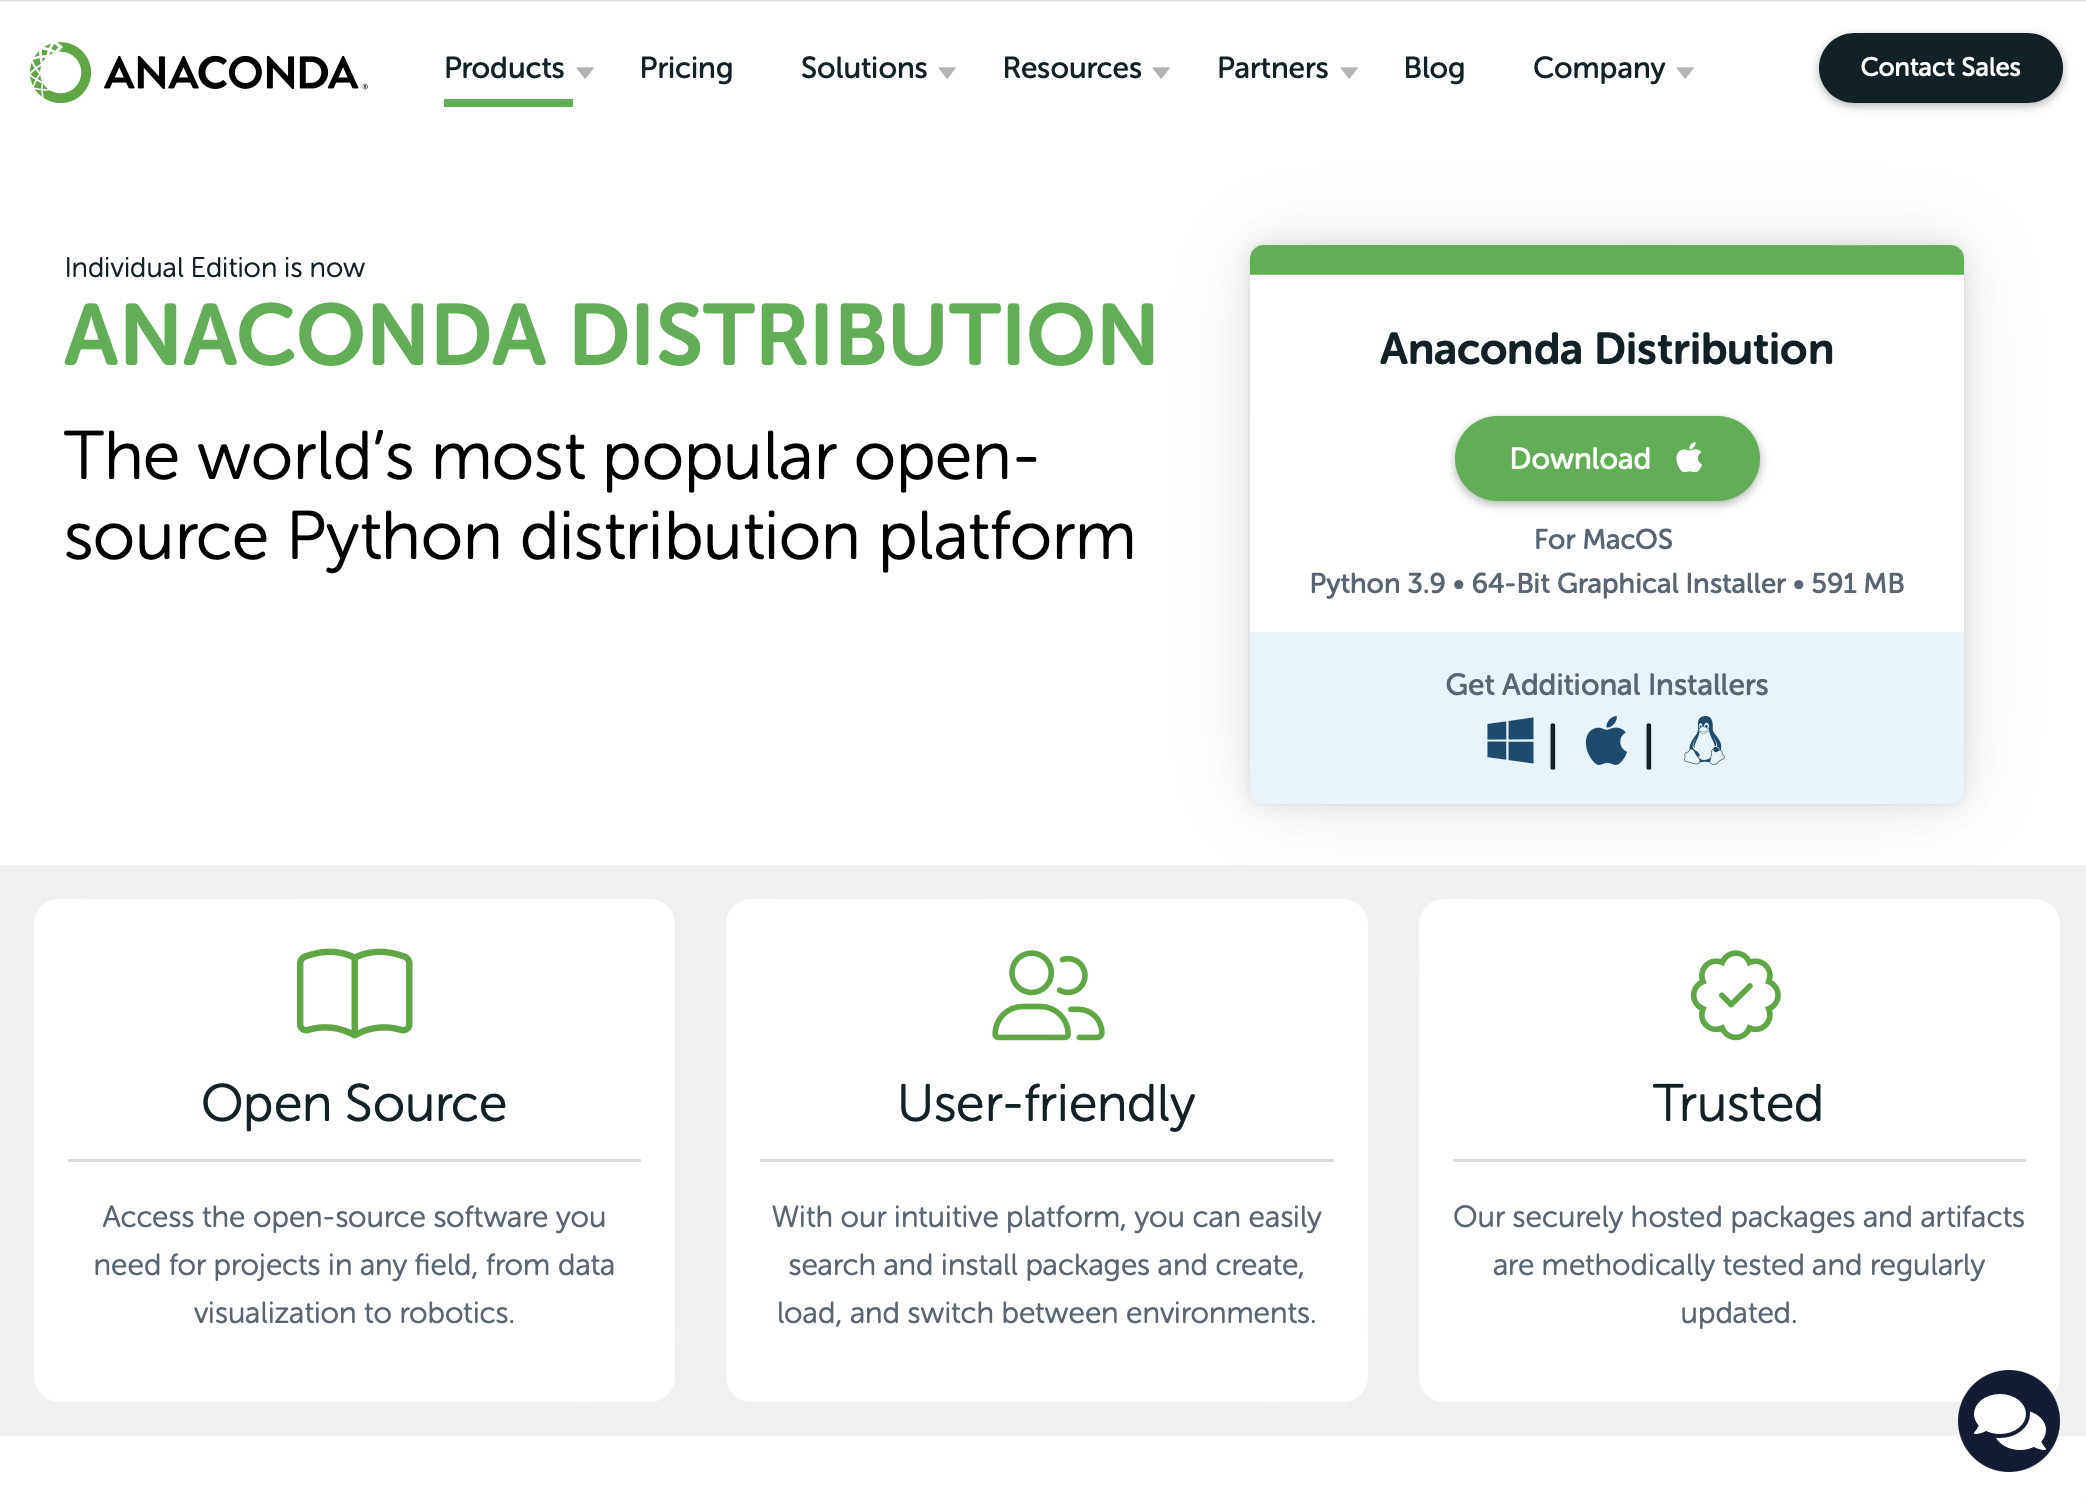
\includegraphics[width=0.75\textwidth]{images/anaconda_distro.png}
	\end{figure}
\end{frame}

\subsection{Installation Procedure for Anaconda}

\begin{frame}[c]{Steps}
	\begin{enumerate}
		\item Downaload the installer for your operating system (unless you have a very old machine running Win, go for the 64-Bit version)
		\item Run the installer
		\begin{itemize}
			\item For Linux: navigate to the folder where you have downloaded the installer as per step 1, open a shell session, then run \texttt{\$ bash ./Anaconda3-XXXX.XX-Linux-x86-64.sh}
			\item For Win and Mac OS: just run the graphical installer downloaded in step 1
		\end{itemize}
		\item Accept the terms proposed by the Anaconda people to use their software, comprising Python, the \texttt{conda} package manager, and a bundle of modules for data science
		\item That's it!
		\begin{itemize}
		\item For Linux users: if you accepted the default installation options, an environmental variable has been created either in your \texttt{.bashrc} or \texttt{.zshrc}. That means you can access the various pieces of software included in the Anaconda installation (e.g., Anaconda Navigator) from a shell session
		\item For Win and Mac OS users: the various pieces of software included in the Anaconda installation are available from the menu of your system
		\end{itemize}
	\end{enumerate}
\end{frame}

\section{How Python Runs Programs}


\section{How We Run Python Programs}

\subsection{Non-Interactive Approach}

\begin{frame}[fragile]{Script Preparation $\rightarrow$ Script Run}
	\begin{columns}[t]
		\begin{column}{0.5\textwidth}		
		\textbf{Step 1: script preparation}	
		
		\vspace{1em}
		
		The below displayed Python code achieves two things:i) it prints the string object ``Bazinga!'', and ii) it prints the resul of the algebraic operation $4 + 2$. Note that all lines starting with \texttt{\#} are not considered Python code --- instead, they are comments that illustrate/explain the logic of the script.
		
		\rule{\textwidth}{1pt}
		\scriptsize
		\begin{minted}{python}
# This prints a string object
print("Bazinga")
# This prints the result of an algebraic operation
print(2 + 4)
	    \end{minted}
		\rule{\textwidth}{1pt}
		
		\end{column}
		\begin{column}{0.5\textwidth}
		\textbf{Step 2: script run}	
		
		\vspace{1em}
		
	\begin{figure}
		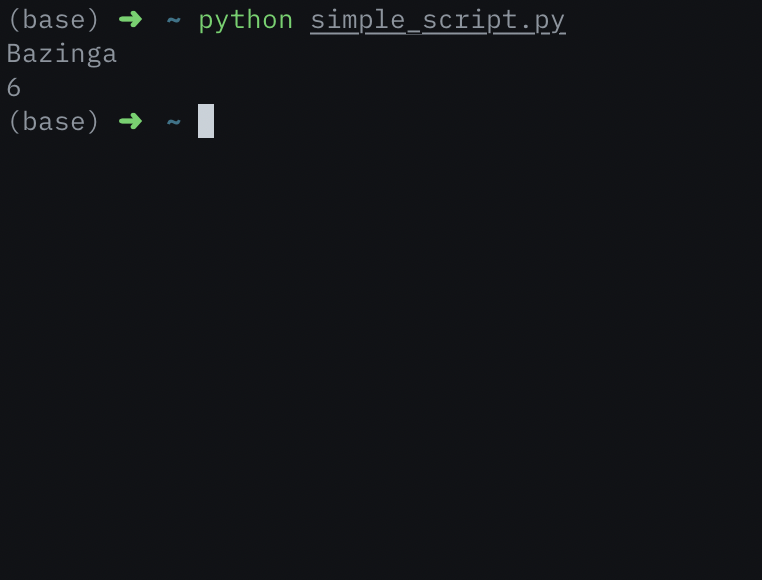
\includegraphics[width=0.92\textwidth]{images/simple_script}
	\end{figure}
		\end{column}
	\end{columns}
\end{frame}

\subsection{Interactive Approach}

\begin{frame}{Running a Python Shell in the Terminal}
		\begin{figure}
			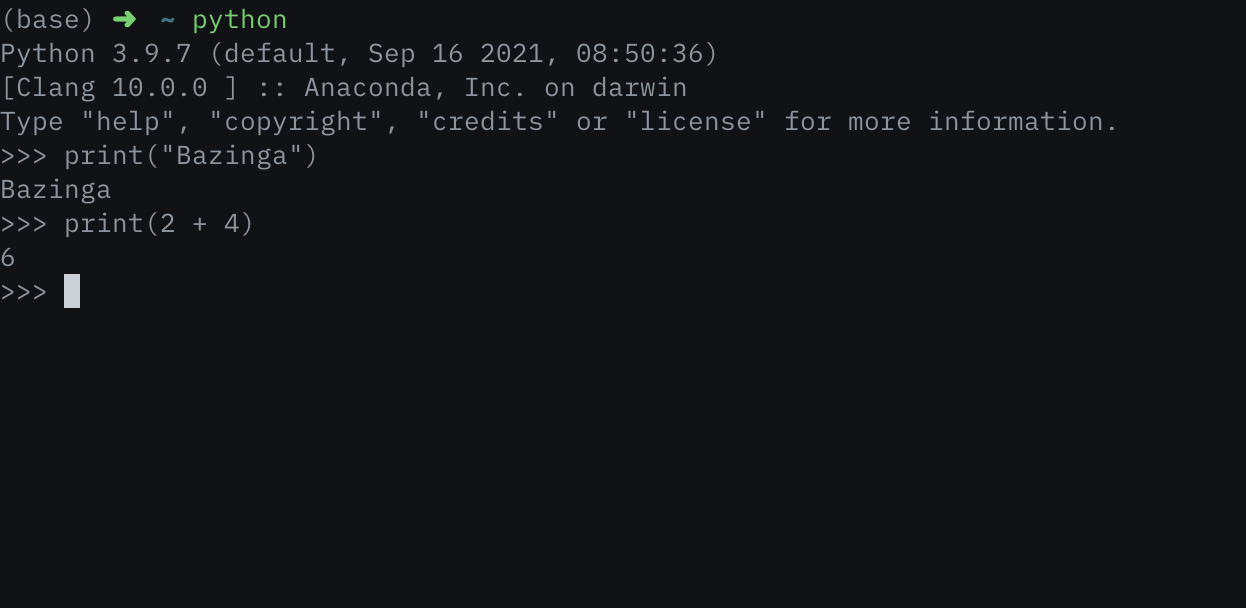
\includegraphics[width=0.9\textwidth]{images/python_session}
		\end{figure}
\end{frame}

\begin{frame}{Running an IPython Shell in the Terminal}
		\begin{figure}
			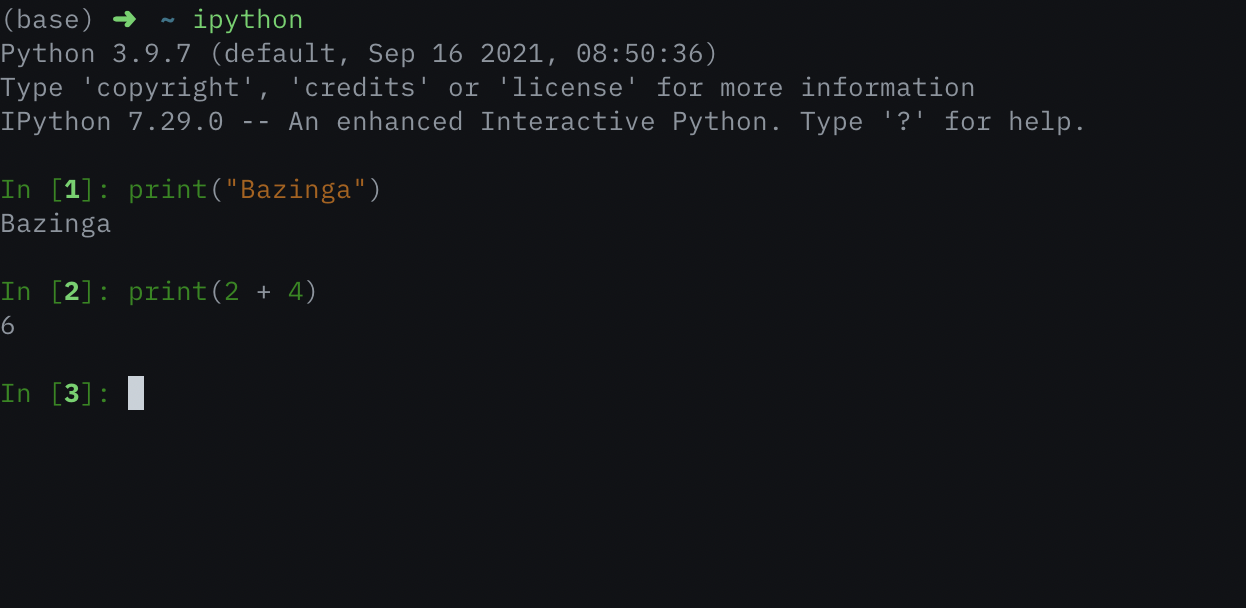
\includegraphics[width=0.9\textwidth]{images/ipython_session}
		\end{figure}
\end{frame}

\begin{frame}[t]{Running a Python IDE}

	\begin{columns}[t]
	
	\begin{column}{0.45\textwidth}

	There are plenty of Python IDEs in the market, including:
	
	\begin{itemize}
		\item Colab (online)
		\item IDLE
		\item Datalore (online)
		\item Jupyter/Jupyterlab
		\item PyCharm
		\item Spyder
		\item Thonny
		\item Wing
	\end{itemize}
	
	\end{column}
	
	\begin{column}{0.45\textwidth}
	
	By installing a couple of plugins, the following (advanced) text editors can turn into Python IDEs:
	
	\begin{itemize}
		\item Emacs
		\item Vim/Neovim
		\item VSCode
	\end{itemize}
	
	\end{column}
	
	\end{columns}
\end{frame}

\begin{frame}{Interactive Python Coding with Jupyter}
		\begin{figure}
			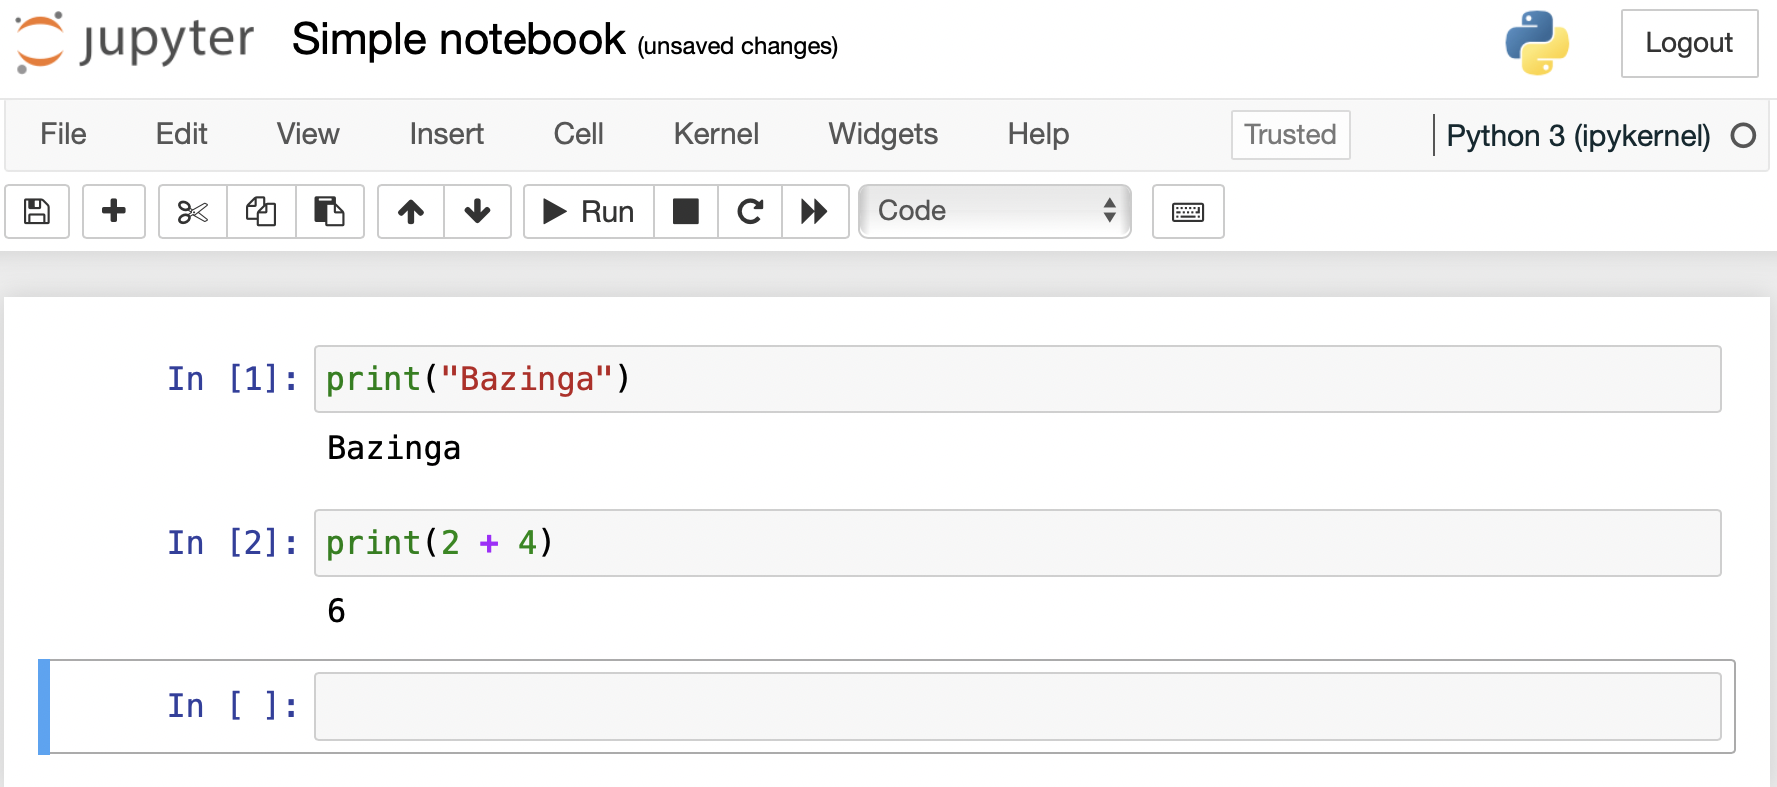
\includegraphics[width=0.9\textwidth]{images/jupyter}
		\end{figure}
\end{frame}

\begin{frame}{Interactive Python Coding with VSCode}
		\begin{figure}
			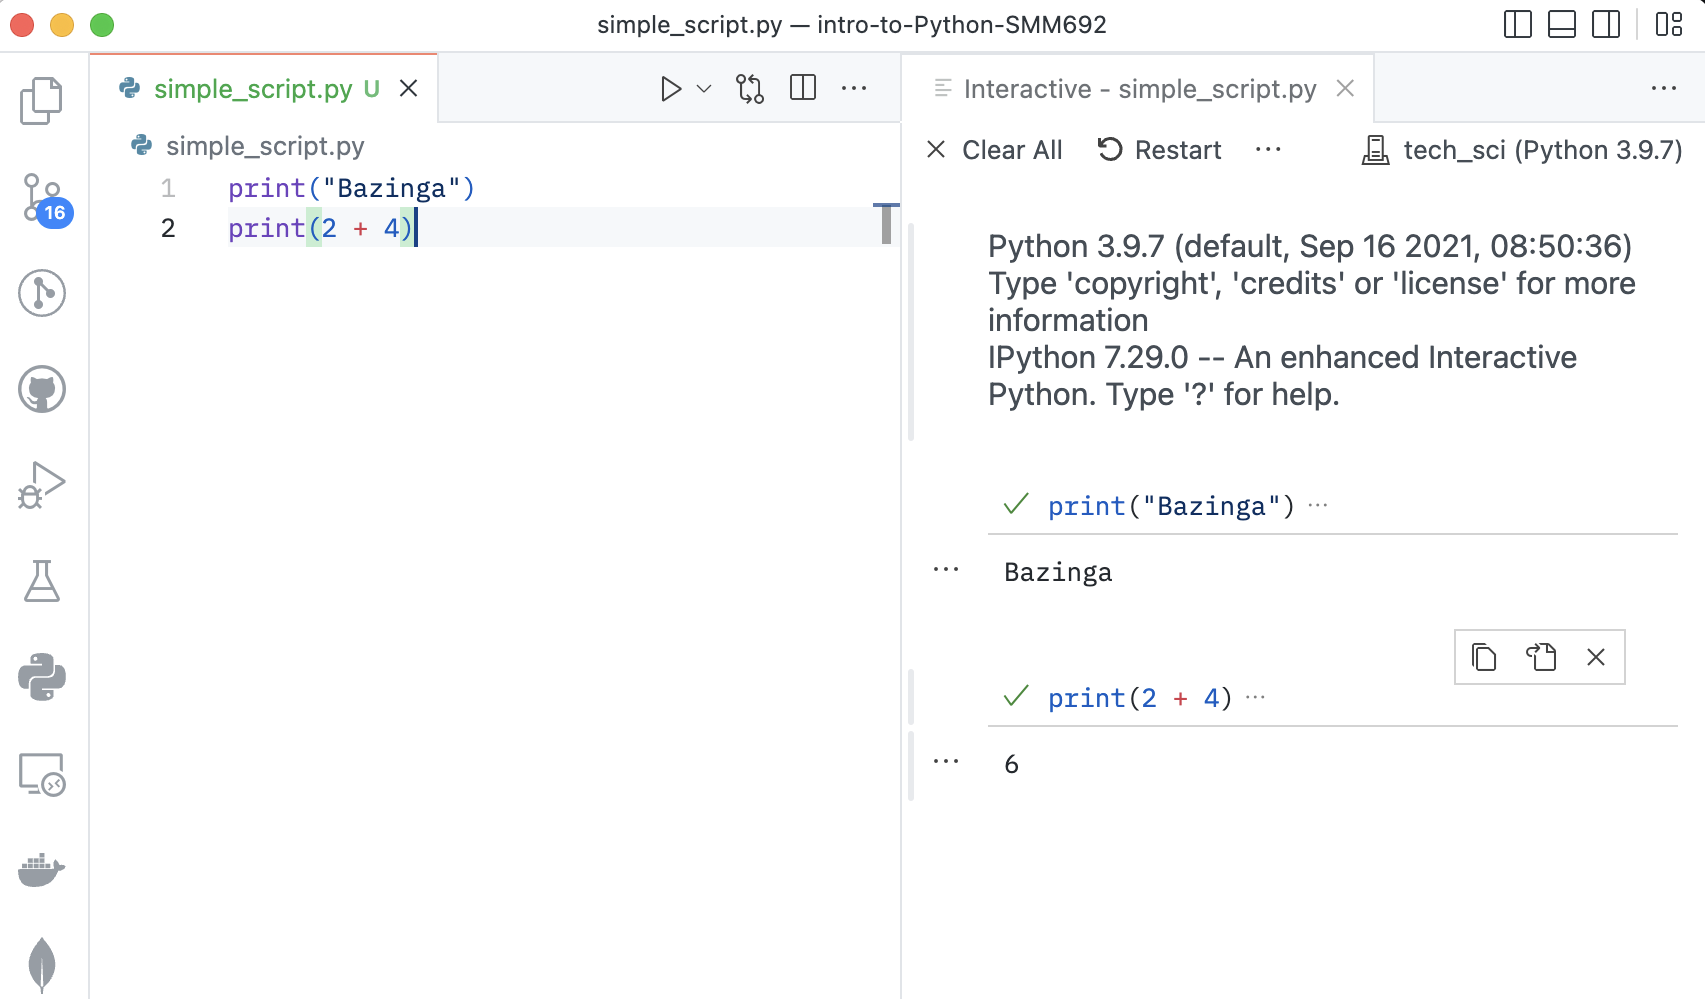
\includegraphics[width=0.9\textwidth]{images/vscode}
		\end{figure}
\end{frame}

\begin{frame}{Interactive Python Coding in Jupyter with VSCode}
		\begin{figure}
			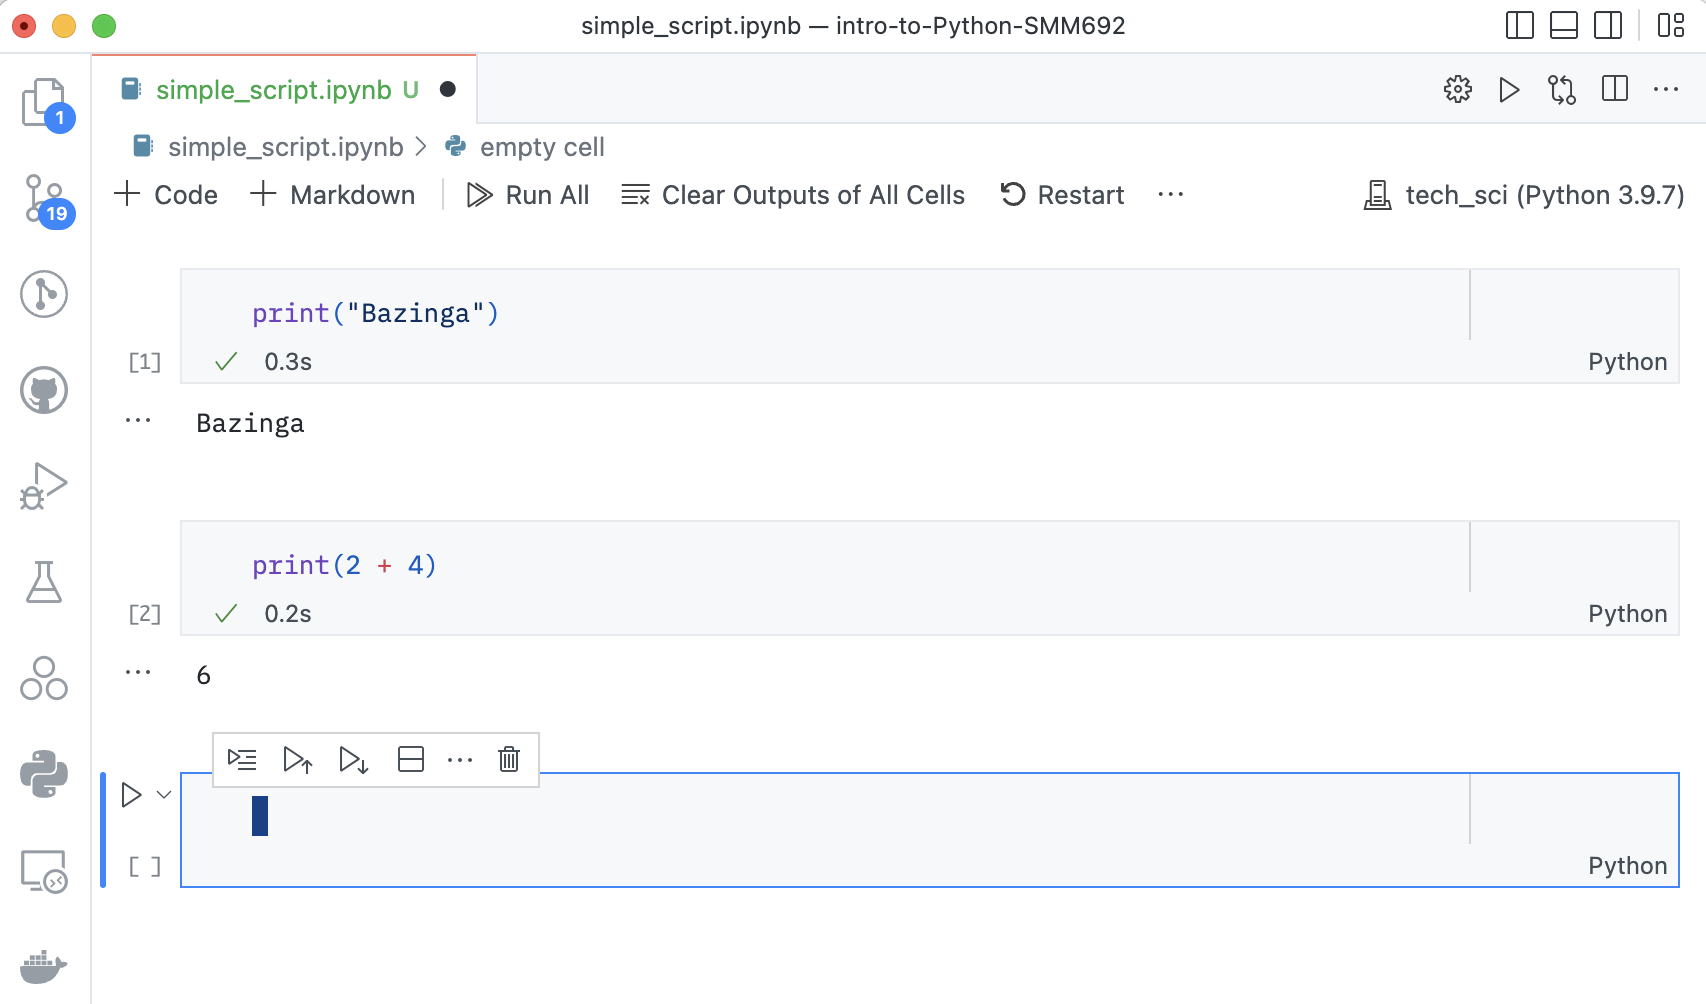
\includegraphics[width=0.9\textwidth]{images/jupyter_in_vscode}
		\end{figure}
\end{frame}

\section{Managing Python Environments}


\section{Collaborative and Versioning Tools}

\end{document}